% !TeX spellcheck = cs_CZ
% options:
% thesis=B bachelor's thesis
% thesis=M master's thesis
% czech thesis in Czech language
% slovak thesis in Slovak language
% english thesis in English language
% hidelinks remove colour boxes around hyperlinks
\RequirePackage{color}
\definecolor{gr1}{RGB}{0,153,51}
\documentclass[thesis=M,czech]{FITthesis}[2012/06/26]


\usepackage[utf8]{inputenc} % LaTeX source encoded as UTF-8

\usepackage{graphicx} %graphics files inclusion
\usepackage{amsmath} %advanced maths
\usepackage{amssymb} %additional math symbols
\usepackage{rotating}

\usepackage{dirtree} %directory tree visualisation
% % list of acronyms
% \usepackage[acronym,nonumberlist,toc,numberedsection=autolabel]{glossaries}
% \iflanguage{czech}{\renewcommand*{\acronymname}{Seznam pou{\v z}it{\' y}ch zkratek}}{}
% \makeglossaries
 

\newcommand{\tg}{\mathop{\mathrm{tg}}} %cesky tangens
\newcommand{\cotg}{\mathop{\mathrm{cotg}}} %cesky cotangens

% % % % % % % % % % % % % % % % % % % % % % % % % % % % % % 
% ODTUD DAL VSE ZMENTE
% % % % % % % % % % % % % % % % % % % % % % % % % % % % % % 

\department{Katedra geomatiky     }
\acknowledgements{Studijní program Geodézie a kartografie}

\title{Kartografická vizualizace vývoje území v údolí řeky Otavy v okolí Strakonic}
\authorGN{Petra} %(křestní) jméno (jména) autora
\authorFN{Pasovská} %příjmení autora
\authorWithDegrees{Bc. Petra Pasovská} %jméno autora včetně současných akademických titulů
\supervisor{Ing. Tomáš Janata, Ph.D.}
\acknowledgements{Děkuji Ing. Tomáši Janatovi, Ph.D., za odborné vedení práce a cenné rady, které mi pomohly tuto práci zkompletovat. Velké díky také patří mé rodině a přátelům, kteří mi byli po dobu zpracování velkou oporou.}
\abstractCS{Abstrakt CZ}
\abstractEN{Abstrakt EN}
\placeForDeclarationOfAuthenticity{V~Praze}
\declarationOfAuthenticityOption{1} %volba Prohlášení (číslo 1-6)
\keywordsCS{klicova slova \newpage}
\keywordsEN{keywords}

\begin{document}

% \newacronym{CVUT}{{\v C}VUT}{{\v C}esk{\' e} vysok{\' e} u{\v c}en{\' i} technick{\' e} v Praze}
% \newacronym{FSv}{FSv}{Fakulta stavebn{\' i}}

\begin{introduction}
Úvod


\end{introduction}

\chapter{Rešerše literatury}
bla bla



\chapter{Otava}
Zlatonosná a perlorodá řeka. Těmito přívlastky bývá Otava často označována. Keltové rýžovali zlato na Otavě již před dvěma tisíci lety. Díky tomu si také vysloužila svůj název – Otava\footnote{V keltštině Atavah či Watawah}, tedy Bohatá řeka. Druhý přívlastek si Otava vysloužila hojným výskytem perlorodek. Ty se v 15. a 16. století začaly chovat v Horažďovicích za velké podpory jezuitů. V roce 1809 a 1818 se výlovu perlorodek zúčastnil i císař František I. Populace perlorodek však rapidně klesla kvůli znečištění a nepříznivým změnám půdních a vegetačních poměrů a perlorodky byly na Otavě téměř vyhubeny. \cite{SMOOS}


\section{Hydrologie}
Ústředním tématem této práce je řeka Otava. Z toho důvodu je vhodné prozkoumat i vědu, která se řekami zabývá. Jedná se o hydrologii.


Hydrologie je věda, která se zabývá zkoumáním zákonitostí výskytu, oběhu, časového a prostorového rozložení zásob vody na Zemi, jejího vzájemného působení s biotickými a abiotickými faktory s ohledem na její fyzikální, chemické a biologické vlastnosti. 


S hydrologií úzce souvisí i hydrogeografie, což je jedna z dílčích fyzickogeografických věd zabývající se vztahem mezi vodními útvary na pevnině a ostatními krajinotvornými prvky. Od hydrologie se liší tím, že používá převážně geografické metody při studiu hydrologických jevů a procesů. 


Hydrologii lze rozdělit podle dvou hlavních kritérií - dle pracovních metod a dle prostředí. Podle pracovních metod se rozděluje na hydrometrii a hydrografii. Hydrometrie zahrnuje měření mechanických, fyzikálních, chemických a biologických jevů ve vodních systémech, hydrografie popisuje hydrologické jevy, hydrologické prostředí, vlastnosti vodních systémů, třídění zpracování a klasifikaci získaných informací. Podle prostředí se rozděluje na hydrologii pevnin (ta lze následně rozdělit na hydrologii atmosféry, řek, jezer, bažin, podzemních vod a ledovců) a hydrologii oceánů. 

Součástí hydrologie je několik vědních oborů. Za zmínku stojí například hydrometeorologie, hydroklimatologie či hydrogeologie. Přesto není do hydrologie začleněna oceánografie a meteorologie, neboť voda je jen jedním ze zkoumaných aspektů. Hydrologie byla řadu let analyzována v rámci geografie. Oddělila se až v 19. století jako samostatná vědní disciplína hydrologie. 

Počátky studia vody na Zemi však sahají do roku 3000 př. n. l. V té době ve starověkém Egyptě byla sledována hladina Nilu na tzv. nilometrech.\footnote{Nilometr je moderní označení pro stavbu ve starověkém Egyptě pro měření výšky nilských záplav. Mají podobu dlouhé sestupné chodby nebo studny a většinou jsou propojeny s hladinou Nilu. Výška byla určována v loktech.} Podobná pozorování probíhala i v Mezopotámii na řece Eufrat a Tigris nebo v Číně. Vodou se zabývali i řečtí filozofové, zejména Thales z Milétu, Platón či Aristoteles. 


Ústředním tématem této práce je řeka Otava. Z hydrologického hlediska tedy budou blíže prozkoumány jen pojmy a analýza týkající se řek. \cite{definiceHydro} \cite{FGkniha} \cite{hydro_net}


\begin{figure}[h!]
	\centering
	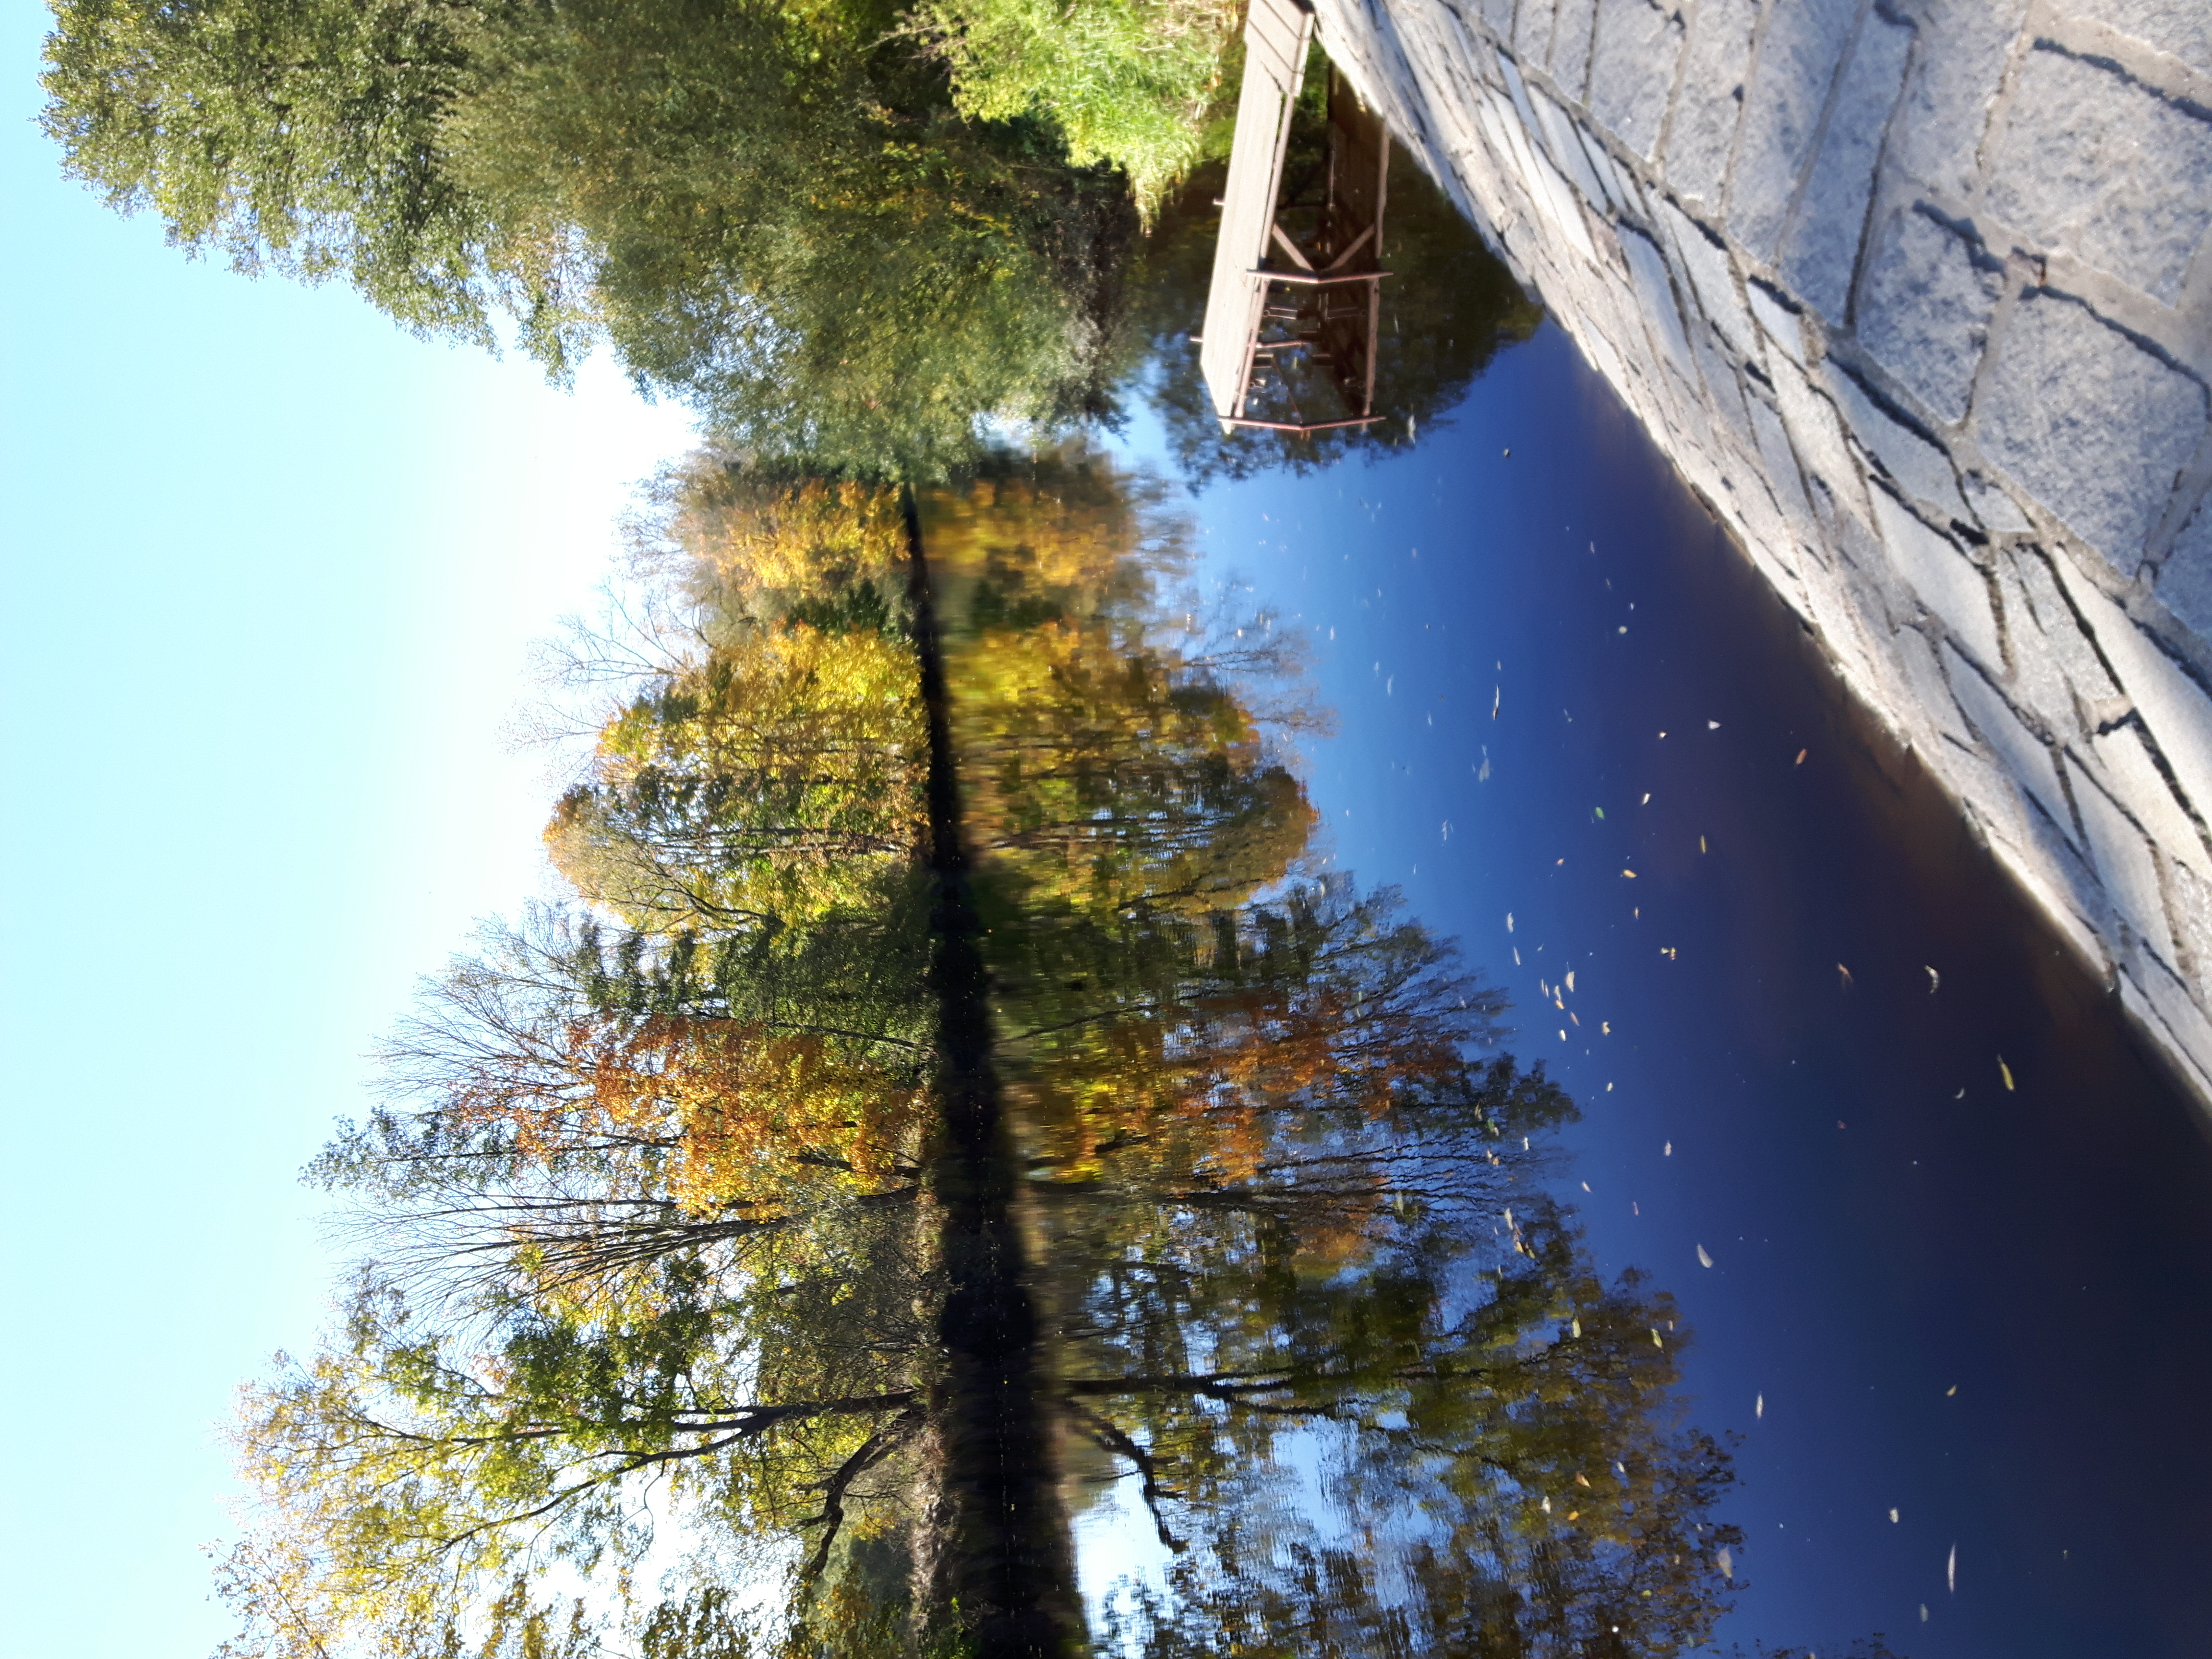
\includegraphics[width=11cm, angle =270]{pics/ot1.jpg}
	\caption{Otava na Podskalí ve Strakonicích na podzim}
	\label{obrazek:ot1}
\end{figure}


\subsection{Vysvětletní základních termínů}
Při hydrologické analýze je vhodná znalost základních pojmů. Ty jsou zde stručně popsány a vysvětleny, neboť jsou v rámci práce často používány. \cite{terminy}


\begin{description}
\item[Pramen:] místo přirozeného výtoku podzemní vody, může být studený nebo termální, v oblastech se sopečnou činností gejzír
\item[Soutok:] místo, kde se setkávají nejméně dva vodní toky
\item[Vodní tok:] voda tekoucí po zemském povrchu v korytě mezi břehy, větší toky jsou označovány jako řeky, menší toky jsou potoky
\item[Říční síť:] půdorysná síť hlavního toku řeky a jejích přítoků, tvar je závislý na geologických a fyzickogeografických podmínkách povodí řeky
\item[Hustota říční sítě:] poměr délky všech toků k ploše povodí
\item[Povodí:] plocha území, ze kterého tok odvádí povrchovou a podpovrchovou vodu
\item[Rozvodí:] hranice mezi jednotlivými povodími
\item[Rozvodnice:] pomyslná čára mezi sousedními povodími
\item[Úmoří:] plocha, ze které se všechna povrchová voda odvádí do moře nebo oceánu
\item[Přítok:] tok nižšího řádu, který se vlévá do toku vyššího řádu
\item[Ústí:] místo, kde se tok vlévá do jiného toku, vodní nádrže či oceánu
\item[Zátopové území:] část území v okolí vodních toků, které je periodicky zaplavované zvýšenými průtoky (pozn.: též inundace)
\end{description}



\subsection{Hydrologická analýza}
V rámci práce byla provedena jednoduchá základní hydrologická analýza. Pro analýzu byla použita data z katalogu DIBAVOD. Pro tvorbu analýzy byl použit software ArcGIS a MS Excel. Analýza byla prováděna dle studijních materiálů Univerzity Karlovy Katedry fyzické geografie a geoekologie. \cite{UK}

Otava vzniká na Šumavě u Čeňkovy Pily soutokem Vydry a Křemelné. Vydra pramení na SZ svahu Luzného ve výšce 1215 m n. m. Díky okolním rašeliništím má Vydra rezavohnědou barvu. Svůj název si nese až po soutoku s Roklanským potokem v obci Modrava\footnote{V některých publikacích se uvádí název Vydra již od Březníku}. Řeka Křemelná pramení v Železnorudské hornatině v přírodní rezervaci Prameniště a severním svahu hory Pancíř (1214 m n. m.). \cite{SMOOS}

\begin{figure}[h!]
	\centering
	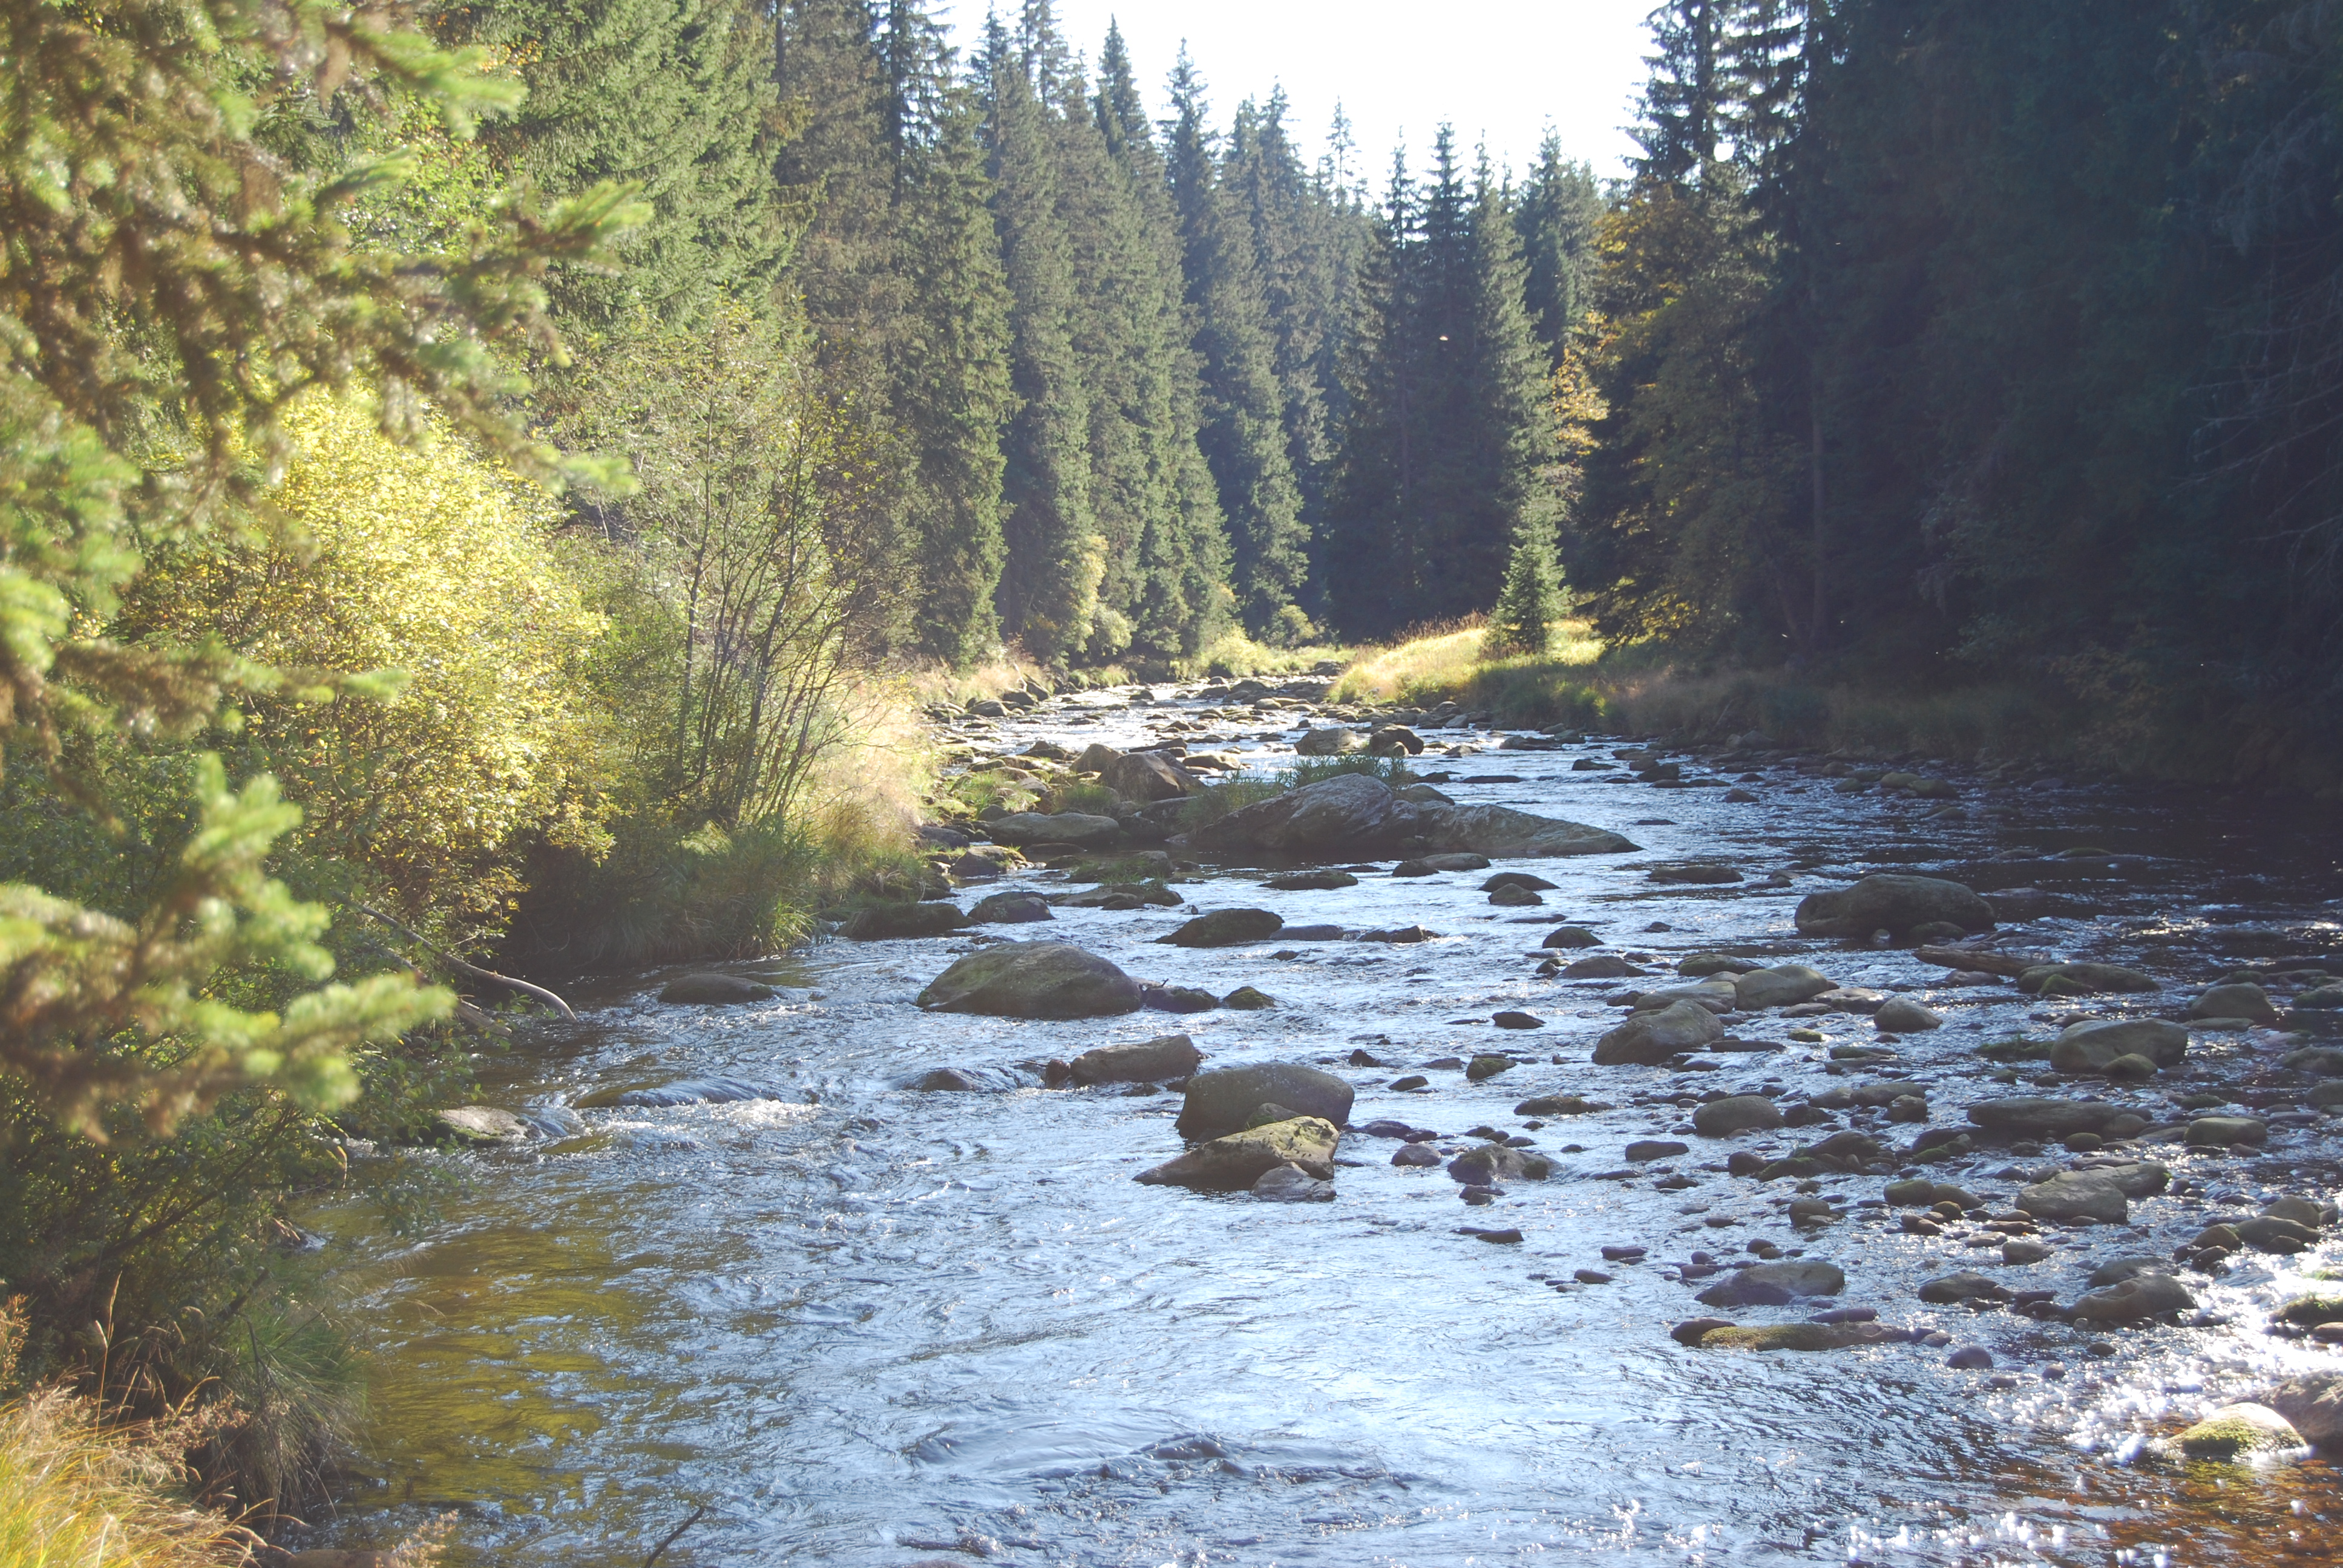
\includegraphics[width=12cm]{pics/vydra.jpg}
	\caption{Řeka Vydra}
	\label{obrazek:ot1}
\end{figure}

Řeka má několik přítoků. Mezi nejznámější patří řeka Ostružná, která ústí do Otavy nedaleko města Sušice. Významným přítokem je řeka Volyňka. Na soutoku Volyňky a Otavy se nachází město Strakonice. Před Pískem do Otavy vtéká Blanice. Poslední významnou řekou je Lomnice, která je levostranným přítokem Otavy. 

Otava je levostranným přítokem Vltavy, do níž se vlévá pod hradem Zvíkov poblíž Orlické přehrady. Povodí Otavy spadá do úmoří Severního moře (Otava~$\rightarrow$~Vltava~$\rightarrow$~Labe~$\rightarrow$~Severní moře ). 


Pokud bychom chtěli popsat řeku čísly, pak její délka je 111.7 km a plocha povodí 3841 km$^2$. Ze znalosti délky a plochy povodí můžeme dané povodí popsat dle vzorce pro charakteristiku povodí:\\


$$\alpha = \frac{P}{L^2} = \frac{3841}{111.7^2} = 0.31$$ \\


Povodí lze tedy označit jako vějířovité. Dále je možné vypočítat Graveliuv koeficient a koeficient protáhlosti povodí. Pro výpočet Graveliova koeficientu je zapotřebí znát délku rozvodnice $L_R$\footnote{Délka rozvodnice byla určena v software ArcGIS výpočtem geometrie prvku}. \\

$Gravieluv\ koeficient: K_G = \frac{L_R}{2 \sqrt{P \cdot \pi}} = \frac{412}{2\sqrt{3841\cdot \pi}} = 1.88$ \\

$Koeficient\ protáhlosti\ povodí: R_E = \frac{2\cdot \sqrt{P / \pi}}{L} = \frac{2 \cdot \sqrt{3841 / \pi}}{111.7} = 0.63 $ \\



Ze znalosti délky všech toků jsme schopni vypočítat hustotu říční sítě.\\

$Hustota\ říční\ sítě: r = \frac{\sum L}{P} = \frac{a}{b} $


\section{Kulturní a historické informace o ??? vymyslet pěkný název}
Otava protéká několika historicky významnými městy. Mezi nejvýznamnější města, kterými řeka protéká, patří Sušice, Horažďovice, Strakonice a Písek. Blíže popsány jsou také Žichovice z důvodu nedaleké zříceniny hradu Rabí.

\subsection{Sušice}


\subsection{Žichovice}

\subsection{Horažďovice}



\subsection{Strakonice}


\subsection{Písek}

\section{Události na Otavě}
\subsection{Rýžování zlata}

\subsection{Povodeň v roce 2002}

\chapter{Použitá data}
\section{Kartografické podklady}
\subsection{Císařské povinné otisky stabilního katastru}

\subsection{Katastrální mapa}


\section{Stavební plány Strakonického hradu}


\section{Fotodokumentace}

\chapter{Zpracování dat}
\section{Tvorba 3D modelu Strakonického hradu}

\section{Georeferencování}


\chapter{Prezentace na webových stránkách}


\chapter{Diskuze}



\begin{conclusion}
Závěr
\end{conclusion}

\bibliographystyle{csn690}
\bibliography{mybibliographyfile}

\appendix

\chapter{Seznam použitých zkratek}
% seřadit podle abecedy
% \printglossaries
\begin{description}
	\item[DIBAVOD] Digitální báze vodohospodářských dat

\end{description}



\chapter{Obsah přiloženého CD}

\begin{figure}
	\dirtree{%
		.1 readme.txt\DTcomment{stručný popis obsahu CD}.
		.1 grafy\DTcomment{složka obsahující výsledné grafy}.
		.1 rastry\DTcomment{složka obsahující testované rastry}.
		.1 rozklad.m\DTcomment{skript na výpočet rozkladu RGB barev}.
		.1 LaTex\DTcomment{zdrojová forma práce ve formátu \LaTeX{}}.	
		.1 text\DTcomment{text práce}.
		.2 BP\_Pasovska\_Petra\_2017\DTcomment{text práce v PDF}.	
	}
\end{figure}

\end{document}